\documentclass[10pt,landscape]{standalone}
\usepackage{pgfplots}
\pgfplotsset{compat=1.18}

\begin{document}

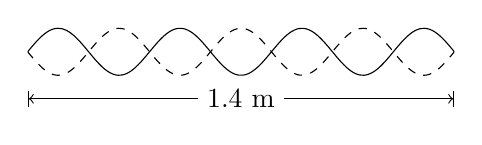
\begin{tikzpicture}

  \begin{axis}[
    width=7cm, height=3cm,
    declare function ={myfunc(\x) = 0.2*sin(deg(2*pi*\x/4));},
    axis y line = none,
    axis x line = none,
    xmin=0, xmax=14,
    ymin=-.6, ymax=.35,
  ]
     \addplot[smooth, domain={0:14},samples=100] {myfunc(x)};
     \addplot[smooth, dashed, domain={0:14},samples=100] {-myfunc(x)};
     \draw[|<->|] (0,-0.4) -- (14,-0.4) node[midway, fill=white] {1.4 m};
  \end{axis}

\end{tikzpicture}


\end{document}